\section{Durchführung}
\label{sec:Durchführung}

Der Versuchsaufbau besteht aus einer Drehschieberpumpe zur Erzeugung des Vakuums und dazugehörigem Vakuumbehälter.
In diesem Behälter befindet sich die eigentliche Messapperatur.
Diese ist in Abbildung \ref{fig:aufbau} dargestellt.
Die Einheiten sind jeweils $\si{\milli\meter}$ für alle Längen.
Die \alphat~werden, nach dem Austritt aus der Quelle, im Kollimator parallel ausgerichtet.
Anschließend streuen sie an einer dünnen Folie, im Laufe des Versuches werden verschiedene Materialien und Dicken verwendet.

\begin{figure}[ht]
  \centering
  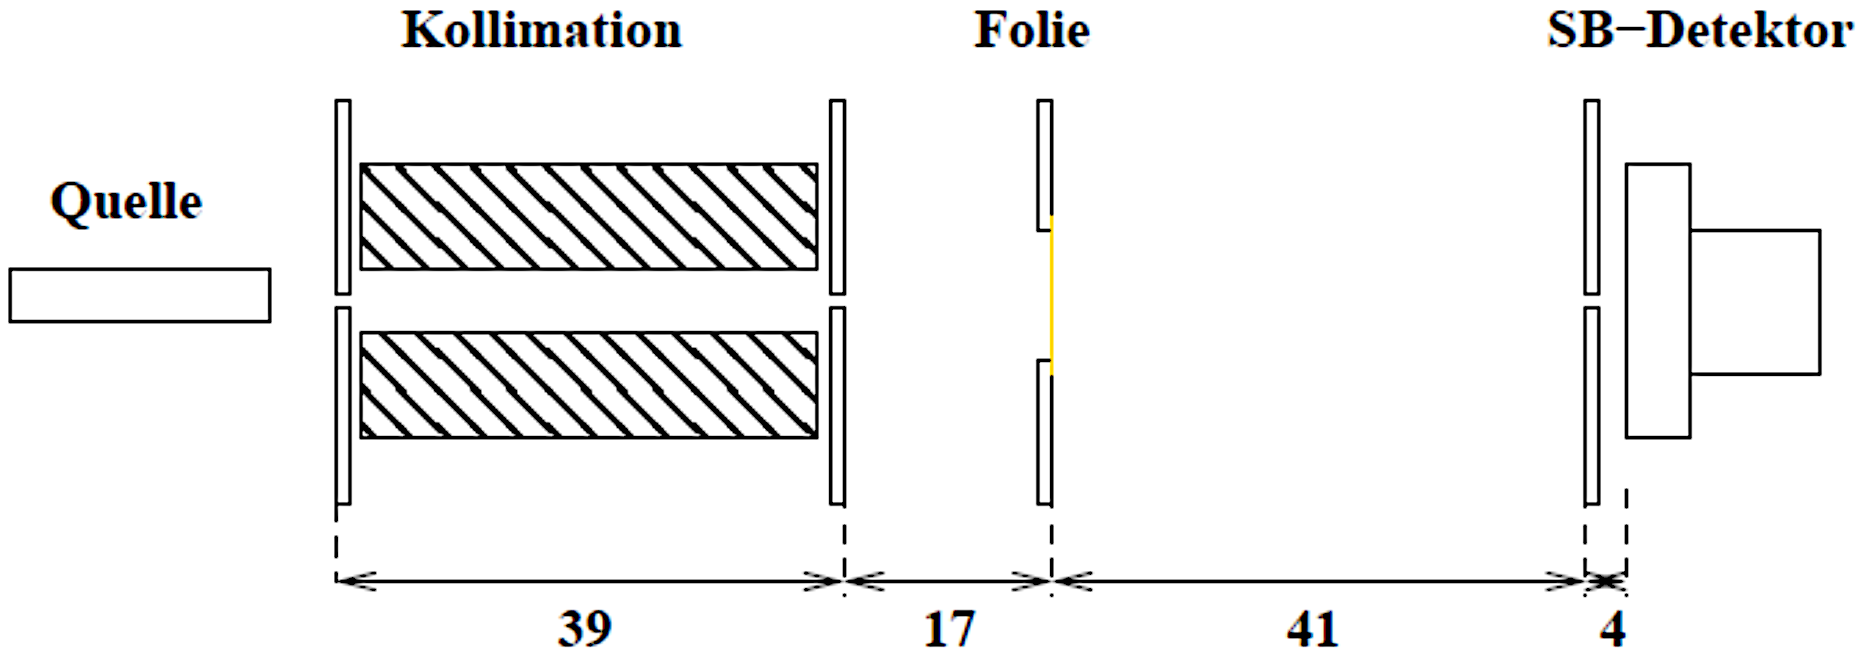
\includegraphics[width=0.8\textwidth]{images/aufbau.png}
  \caption{Skizze der Messapperatur. Längenangaben in Millimetern. \cite{anleitung}}
  \label{fig:aufbau}
\end{figure}

Der SB-Detektor kann um die Folie gedreht werden.
Die Stellung in Abbildung~\ref{fig:aufbau} entspricht $φ=\SI{0}{\degree}$.
Die Spannung des SB-Detektors bleibt während aller Messungen bei
$U_\text{det} = \SI{12}{\volt}$.

Das Ausgangsignal wird je nach Messung mit einem Oszilloskop dargestellt oder in einem Zählwerk detektiert.

In der ersten Messungen werden die Pulse des Detektors auf dem Oszilloskop zeitlich aufgelöst beobachtet.
Zuerst die unverstärkten und dann die, durch dem Zähler vorgeschaltetem Verstärker, verstärkten.

Der Einfluss der Foliendicke auf die Zählrate, in Kombination mit dem Kammerdruck, wird in der zweiten Messung bestimmt.
Hierfür wird die Impulshöhe auf dem Oszilloskop im Bereich von $\SI{0.04}{\milli\bar}$ bis $\SI{200}{\milli\bar}$ notiert.
Jeweils eine Messreihe für eine $\SI{2}{\micro\meter}$ Goldfolie und eine Messreihe ohne Folie.
Da die Impulshöhen schwanken wird eine maximale und minimale Amplitude genommen.

Die Winkelabhängigkeit der Zählrate wird, im Vakuum, für die 2 und $\SI{4}{\micro\meter}$ Goldfolie bestimmt.
Die Integrationszeit wird so gewählt, dass die Zählung ungefähr ein Ergebnis von $\num{1111}$ bringt.

Die Messung Nummer vier erfolgt zur Bestimmung des Einflusses von Mehrfachstreuungen.
Es wird bei einem festen Winkel für verschiedene Foliendicken die Anzahl an gestreuten Teilchen gemessen.

In der letzten Messung wird das Material der Folie geändert.
Bei einem Winkel von $\SI{20.1}{\degree}$ werden die Folien in Tabelle \ref{tab:folien}, bei einer Integrationszeit von
$\SI{300}{\second}$, verwendet:
\begin{table}
  \centering
  \caption{Verwendete Folien für die Z-Abhängigkeit.}
  \label{tab:folien}
  \begin{tabular}{c S[table-format=1.0]}
    \toprule
    {Material} & {Foliendicke$\:/\:\si{\micro\meter}$} \\
    \midrule
    Gold      & 4 \\
    Aluminium & 3 \\
    Bismut    & 2 \\
    \bottomrule
  \end{tabular}
\end{table}
